\chapter{Grundlagen}
\label{ch: Grundlagen}
	Für ein besseres Verständnis, der in Kapitel Konzept... angewandten Methoden, werden anbei die Grundlagen behandelt. Informationen zu der verwendeten Hard- und Software wurden bereits in der vorangegangenen Bachelorarbeit vermittelt. Aufgrund Anforderung A... ist während der praktischen Anwendung keine Änderung der Hardware vorgesehen.
 
	
 	\section{Neuronale Netze}
	\label{sec: ROS}
	
	Das Neuronennetz des menschlichen Gehirns dient als Vorbild für künstliche, neuronale Netze (KNN). Diese werden heutzutage als Lösung diverser Anwendungsprobleme angewendet, in denen komplexe Strukturen und Muster aus großen Datenmengen erkannt werden sollen. Das in diesem Projekt zugrundeliegende Bildverarbeitungsproblem besitzt die beschriebenen Eigenschaften und eignet sich somit für den Einsatz zur Erkennung von Personen. Anders als bei den meisten programmierten Applikationen ist die Ausgabe von KNN's lediglich probabilistisch. Beim vorliegenden, autonomen Logistikfahrzeug werden zur Personenerkennung derartige neuronale Netze verwendet.
	
		\subsection{Eigenschaften von neuronalen Netzen}
		\label{subsec: Eigenschaften von neuronalen Netzen}
		Das Grundlage für die Eingabe in ein neuronales Netz ist die Skalierung der vorliegenden Daten auf eine definierte Größe. Diese wäre beispielsweise bei einem Anwendungsfall mit einer Audiospur die Frequenzspektren oder bei einem Bildverarbeitungsproblem die Pixel eines Bildes. Die skalierten Daten werden in einem Tensor gegeben der die Dimensionen der Eingabe hat. Somit unterteilt sich ein Bild in die drei Dimensionen, die Höhe, die Weite und die Farbwerte der Primärfarben pro Pixel.\\
		
		\begin{figure}[H]
			\centering
			\begin{tikzpicture}[
				init/.style={
					draw,
					circle,
					inner sep=2pt,
					font=\Huge,
					join = by -latex
				},
				squa/.style={
					draw,
					inner sep=2pt,
					font=\Large,
					join = by -latex
				},
				start chain=2,node distance=13mm
				]
				\node[on chain=2] 
				(x2) {$x_2$};
				\node[on chain=2,join=by o-latex] 
				{$w_2$};
				\node[on chain=2,init] (sigma) 
				{$\displaystyle\Sigma$};
				\node[on chain=2,squa,label=above:{\parbox{2cm}{\centering Aktivierungs-funktion}}] 
				{$f$};
				\node[on chain=2,label=above:Ausgabe,join=by -latex] 
				{$y$};
				\draw[fill=black](1,-0.425)circle(1pt);
				\draw[fill=black](1,-0.75)circle(1pt);
				\draw[fill=black](1,-1.075)circle(1pt);
				\begin{scope}[start chain=1]
					\node[on chain=1] at (0,1.5cm) 
					(x1) {$x_1$};
					\node[on chain=1,join=by o-latex] 
					(w1) {$w_1$};
				\end{scope}
				\begin{scope}[start chain=3]
					\node[on chain=3] at (0,-1.5cm) 
					(x3) {$x_n$};
					\node[on chain=3,label=below:Gewichte,join=by o-latex] 
					(w3) {$w_n$};
				\end{scope}
				%\node[label=above:\parbox{2cm}{\centering Bias \\ $b$}] at (sigma|-w1) (b) {};
				
				\draw[-latex] (w1) -- (sigma);
				\draw[-latex] (w3) -- (sigma);
				%\draw[o-latex] (b) -- (sigma);
				
				\draw[decorate,decoration={brace,mirror}] (x1.north west) -- node[left=10pt] {Eingabe} (x3.south west);
			\end{tikzpicture}
			\caption{https://tex.stackexchange.com/questions/132444/diagram-of-an-artificial-neural-network}
			\label{fig: neuron}
		\end{figure}
		Der grundlegende Aufbau eines neuronalen Netzes besteht aus miteinander verbundenen Schichten, die häufig aus Neuronen bestehen. Die typische Struktur eine Neuron ist Abbildung \ref{fig: neuron} zu sehen. Es verarbeitet im wesentlichen eingehende Zahlenwerte $x_n$ und gibt diese durch die Ausgabe $y$ aus. Genauer wird mit den eingehenden Zahlenwerten eine gewichtete Summe gebildet. Diese wird dann auf eine Aktivierungsfunktion angewendet.\\
		
		\begin{equation}
		s=\sum_{j=1}^n w_{ij}x_j
		\label{eq: Gewichtete Summe}
		\end{equation}
		\\
		
		Gleichung \ref{eq: Gewichtete Summe} zeigt das mathematische Modell der gewichteten Summe $s$. Das jeweilige Gewicht $w$ wird mit dem Index $j$ inkrementiert und mit dem dazugehörigen Eingang des Neurons $i$ multipliziert. Alle Produkte werden aufsummiert und ergeben die gewichtete Summe. Es gibt verschiedene Varianten der Aktivierungsfunktion, die je nach Netzart zur Anwendung kommen können. Häufig werden für Aktivierungsfunktion Schwellwertfunktionen angewendet. \\
		
		\tikzset{%
			every neuron/.style={
				circle,
				draw,
				minimum size=1cm
			},
			neuron missing/.style={
				draw=none, 
				%scale=4,
				%rotate=90,
				%yshift=1,
				%text height=0.333cm,
				%execute at begin node=\color{black}$\cdots$
			},
		}
		\begin{figure}[H]
			\centering
			
			
			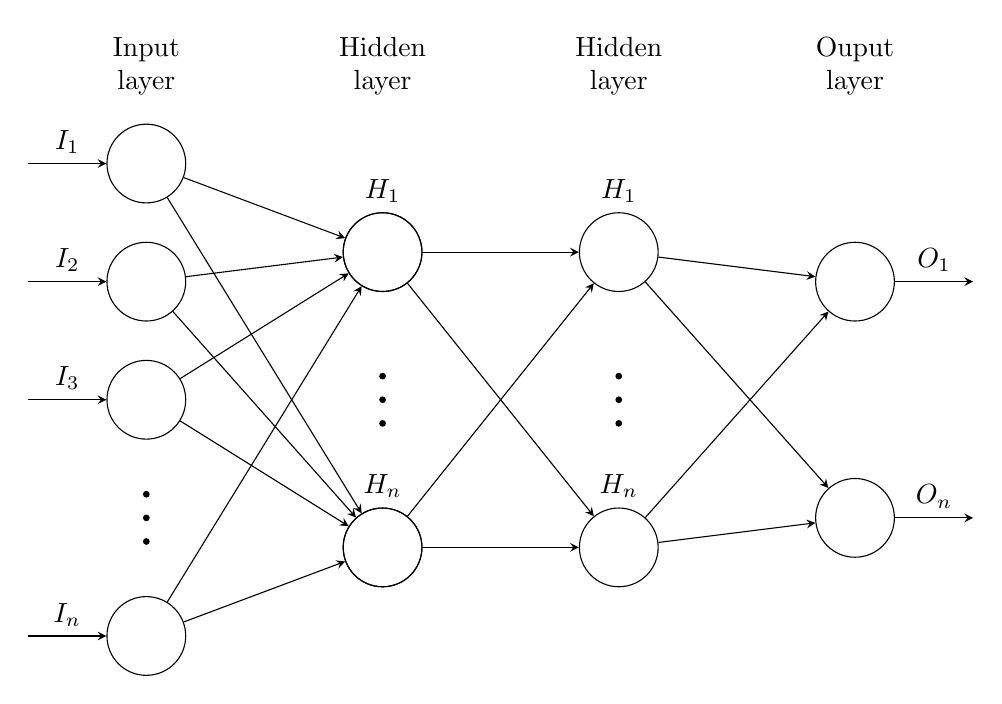
\begin{tikzpicture}[x=1.5cm, y=1.5cm, >=stealth]
				
				\foreach \m/\l [count=\y] in {1,2,3,missing,4}
				\node [every neuron/.try, neuron \m/.try] (input-\m) at (0,2.5-\y) {};
				
				\foreach \m [count=\y] in {1,missing,2}
				\node [every neuron/.try, neuron \m/.try ] (hidden1-\m) at (2,2-\y*1.25) {};
				
				\foreach \m [count=\y] in {1,missing,2}
				\node [every neuron/.try, neuron \m/.try ] (hidden1-\m) at (2,2-\y*1.25) {};
				
				\foreach \m [count=\y] in {1,missing,2}
				\node [every neuron/.try, neuron \m/.try ] (hidden2-\m) at (4,2-\y*1.25) {};
				
				\foreach \m [count=\y] in {1,missing,2}
				\node [every neuron/.try, neuron \m/.try ] (output-\m) at (6,1.5-\y) {};
				
				\foreach \l [count=\i] in {1,2,3,n}
				\draw [<-] (input-\i) -- ++(-1,0)
				node [above, midway] {$I_\l$};
				
				\foreach \l [count=\i] in {1,n}
				\node [above] at (hidden1-\i.north) {$H_\l$};
				
				\foreach \l [count=\i] in {1,n}
				\node [above] at (hidden2-\i.north) {$H_\l$};
				
				\foreach \l [count=\i] in {1,n}
				\draw [->] (output-\i) -- ++(1,0)
				node [above, midway] {$O_\l$};
				
				\foreach \i in {1,...,4}
				\foreach \j in {1,...,2}
				\draw [->] (input-\i) -- (hidden1-\j);
				
				\foreach \i in {1,...,2}
				\foreach \j in {1,...,2}
				\draw [->] (hidden1-\i) -- (hidden2-\j);
				
				\foreach \i in {1,...,2}
				\foreach \j in {1,...,2}
				\draw [->] (hidden2-\i) -- (output-\j);
				
				\foreach \l [count=\x from 0] in {Input, Hidden, Hidden, Ouput}
				\node [align=center, above] at (\x*2,2) {\l \\ layer};
				
				\draw[fill=black](0,-1.3)circle(1pt);
				\draw[fill=black](0,-1.5)circle(1pt);
				\draw[fill=black](0,-1.7)circle(1pt);
				\draw[fill=black](2,-0.3)circle(1pt);
				\draw[fill=black](2,-0.5)circle(1pt);
				\draw[fill=black](2,-0.7)circle(1pt);
				\draw[fill=black](4,-0.3)circle(1pt);
				\draw[fill=black](4,-0.5)circle(1pt);
				\draw[fill=black](4,-0.7)circle(1pt);
				\end{tikzpicture}
				\caption{https://newbiettn.github.io/2016/12/16/tikz/}
				\label{fig: neuronales netz }
		\end{figure}
	
		
		In Abbildung \ref{fig: neuronales netz } ist Grundstruktur eines neuronalen Netzes veranschaulicht. Neuronen sind hier als Kreise dargestellt und bilden in den beispielhaft vertikal veranschaulichten Formationen einzelne Schichten. Hierbei wird zwischen Eingabe-, Zwischen- und Ausgabeschichten unterschieden. Die Eingabeschicht nimmt Informationen in Form von Daten auf und gibt diese an die erste Zwischenschicht weiter. Die Anzahl der Zwischenschichten, oder auch verdeckte Schichten, ist in der Anwendung der neuronalen Netzen variabel. Am rechten Bildrand ist die Ausgabeschicht gezeigt, die die entsprechende Ausgabe des Netzes generiert.  
	
		\subsection{Lernprozess}
		Der Lernprozess von neuronalen Netzen zielt darauf hinaus, einer Netzstruktur ein gewünschtes Verhalten beizubringen. Genauer sollen die in Kapitel... beschriebenen Gewichte modifiziert werden.\\
		
		Zunächst wird zwischen drei Lernverfahren unterschieden, dem unüberwachten, dem bestärkenden und dem überwachten Lernen. Beim unüberwachten Lernen erkennt das Netz selbst Muster und Klassen aus der eingegebenen Menge. Anders als beim unüberwachten Lernen, lernt das Netz beim bestärkten Lernen mit einer Rückmeldung. Diese enthält Informationen darüber, ob ein errechnetes Ergebnis einer Trainingseinheit richtig oder falsch ist. Das überwachte Lernen setzt eine Trainingsmenge voraus, die neben der Eingabedaten auch das dazugehörige korrekte Ergebnis enthält. So wird in der Vorwärtspropagation durch eine Eingabe eine entsprechende Ausgabe erzeugt und diese mit dem korrekten Ergebnis verglichen. Das KNN wird dann mithilfe des aus dem vorangegangenen Vergleich entstandenen Fehler korrigiert.\cite{Kriesel}\\
		
		Die meist genutzte Form des überwachten Lernens ist die Rückwärtspropagierung (engl. Backpropagation) oder Fehlerrückführung genannt \cite{Ertel}. Auch in dieser Masterarbeit werden Netze mithilfe der Rückwärtspropagierung trainiert und in diesem Kapitel genauer erläutert. Die mathematische Grundlage für dieses Lernverfahren sind Gradientenabstiegsverfahren \cite{Kriesel}. Durch die Fehlerrückführung werden Gewichte durch die Ausgabeschicht, die dann als Eingabeschicht genutzt wird, mithilfe des Fehlervektors optimiert \cite{Kriesel}. Dafür ist eine Trainingsmenge in Form eines Datensatzes nötig. Im Falle einer Personenerkennung wäre beispielsweise ein Datensatz aus Bildern von Personen eine geeignete Trainingsmenge. Jedes enthaltene Bild verfügt die Trainingsmenge\\
		
	
		
		\subsection{Evaluation neuronaler Netze}
			
		Die Ausgabe von neuronalen Netzen ist probabilistisch und nicht vorhersehbar. Folglich bestehen diverse Metriken für Evaluationen, die derartige Systeme messbar machen. Im Rahmen dieser Masterarbeit wird die Methode \textit{Precision and Recall} verwendet. Da die Erkennung von Personen auf ein Klassifikationsproblem binärer Natur reduziert werden kann, eignet sich die genannte Herangehensweise. Da die genannte Metrik für diese Arbeit auf ein Bildverarbeitungsproblem angewendet wird, werden die Grundlagen im Folgenden im entsprechenden Kontext vermittelt.\\
		
		\textit{Precision and Recall} ist ein traditionelles Werkzeug zur Evaluation und Leistungsmessung \cite{precisionandrecall}. Der \textit{Recall}-Wert $r(t)$, oder $TPR(t)$ für \textit{Truepositiverate}, beschreibt die Fähigkeit eines System, tatsächlich positive Stichproben zu erkennen. Angewandt auf die Personenerkennung sind Bilder, auf denen Personen zu sehen sind, als tatsächlich positive Stichproben einzustufen. In Gleichung \ref{eq: recall} wird der \textit{Recall}-Wert durch eine Division von allen wahren positiven Werten $TP(t)$ und die Anzahl aller tatsächlich positiven Werte $n_{pos}$ berechnet. Die Variable $t$ definiert den eingestellten Schwellwert. Im Sachkontext ist der Wert als Konfidenz zu betrachten, bei der eine Person als solche klassifiziert wird. Für die Anwendung dieser Methode ist die Kenntnis über negativen Beispielen der Stichprobe nicht notwendig \cite{bildundobjekt}.\\ 
		
		\begin{equation}
		r(t)=TPR(t)=\frac{TP(t)}{TP(t)+FN(t)}
		\label{eq: recall}
		\end{equation}\\
		
		Der \textit{Precision}-Wert $p(t)$ berechnet sich durch das Verhältnis von allen wahren positiven Werten $TP(t)$ durch alle als positiv bewerteten Beispielen $TP(t)$ und $FP(t)$. Durch diesen Wert wird verdeutlicht, wie gut ein System in der Lage ist tatsächlich wahre Werte von tatsächlich falschen Werten zu unterscheiden.\\
		
		\begin{equation}
		p(t)=\frac{TP(t)}{TP(t)+FP(t)}
		\label{eq: precision}
		\end{equation}\\
		
		Häufig muss in der Praxis ein Kompromiss zwischen \textit{Precision} und \textit{Recall} gefunden werden. Dies lässt sich anhand eines Beispiel in der Personenerkennung veranschaulichen. Das System zur Erkennung wird beispielhaft mit einem hohen \textit{Precision}-Wert betrieben. Ein damit verbundener, niedriger \textit{Recall}-Wert ist in der Praxis üblich. Dies führt dazu, dass irrelevanter Bildinhalt selten als Person klassifiert wird. Jedoch kommt es eher häufig vor, dass keine Person detektiert wird obwohl eine zu sehen ist. Legt man nun den Fokus auf einen hohen \textit{Recall}, sinkt der \textit{Precision}-Wert. Personen würden dann zwar häufiger als Person klassifiziert werden, jedoch wird irrelevanter Bildinhalt ebenfalls häufig als Person klassifiziert.
		
		
		
		
		
		
	\section{Objekterkennung}
	\label{sec: Mecanumräder}
	Bei der visuellen Objekterkennung wird ein Objekt, das auf einem Bild gezeigt ist, mit einer gewissen Wahrscheinlichkeit inklusive der Position in der Abbildung erkannt. Die drei Abstraktionsebenen einer solchen Erkennung unterteilen sich in Bildklassifikation, Objektlokalisierung und semantische Segmentierung ...2014Bild. Letzteres kommt in dieser Arbeit nicht zur Anwendung und wird aufgrund dessen im Folgenden nicht behandelt. Die Bildklassifikation beschreibt eine Zuweisung von Objektkategorien zu einem gegebenen Bild. Mithilfe einer Merkmalsextraktion werden Merkmalsvektoren extrahiert und können so in einem Klassifikator berechnet werden. In den folgenden Kapiteln wird auf die in dieser Arbeit eingesetzten Methoden zur Objekterkennung eingegangen. 
	
	
		\subsection{Objekterkennung durch alternative Verfahren}		
		Ein gängiges Verfahren zur Merkmalsextraktion ist das sogenannte Histogram of oriented gradients (HoG). Bei diesem Verfahren werden in einem Bild auftretende Intensitäten geprüft und so Kanten und Ecken als Histogramm gespeichert. Die Support Vektor Maschine ist ein typischer Funktionsapproximator für eine Objektklassifikation. Es handelt sich hierbei um ein Verfahren, das Klassen durch eine sogenannte Hyperebene voneinander trennt. Diese Methode hat sich vor allem aufgrund ihrer kurzen Rechenzeit durchgesetzt.
			
		Wie in Kapitel... beschrieben, soll die Ausgabe einer Objekterkennung auch den Ort eines Objektes enthalten. Für jedes erkannte Objekt wird ein Rechteck in Form von Pixelkoordinaten erzeugt, das den Interessensbereich beschreibt.
	
		\subsection{Objekterkennung durch neuronale Netze}
		
		Die bisher besten Ergebnisse in der Bildverarbeitung im Zusammenspiel mit neuronalen Netzen wurden durch \textit{Convolutional Neural Network} (CNN) ermöglicht \cite{deeplearning}. Anders als bei den bereits erwähnten Methoden geschieht die Merkmalsextraktion hierbei innerhalb des Netzes. Derartige Netzwerke nutzen Faltung zur Verarbeitung der Eingangsdaten statt der üblichen Matritzenmultiplikation \cite{deeplearning}. Der Aufbau eines CNNs setzt sich aus einer Merkmalsextraktion und die darauffolgende Klassifikation zusammen.\\ 
	
		...Bild aufbau cnn schicht
	 	
	
		Eine Einheit der Merkmalsextraktion besteht im grundlegenden Fall aus drei Unterschichten. Dabei können sich diese innerhalb der Merkmalsextraktion hintereinander wiederholen. Dies hat jedoch Einfluss auf die Eigenschaften eines Netzes. Die erste Unterschicht führt Faltungsprozesse mit den Eingangsdaten durch \cite{deeplearning}. Im zweiten Schritt wird eine nichtlineare Aktivierungsfunktion wie der \textit{Rectified Linear Unit} (ReLU) Funktion auf die Ausgangsdaten der Kovolutionsschicht angewendet. In der dritten Unterschicht wird das sogenannte \textit{Pooling} durchgeführt. In einigen Fällen wird die Zusammensetzung der drei Stufen als Kovolutionsschicht bezeichnet \cite{deeplearning}. Im Laufe dieses Kapitels wird auf die Motivationen und der Funktionsweise eines CNNs eingegangen.\\
		
		Es gibt drei Motivationen für die Nutzung von Faltung in einem neuronalen Netz. Hierzu gehören die eingeschränkte Konnektivität, die Parameterverteilung und die äquivariante Darstellung \cite{deeplearning}. Im folgenden Abschnitt werden diese Punkte näher erläutert.\\
		
			\tikzset{%
			every neuron/.style={
				rectangle,
				draw,
				minimum size=1cm
			},
			neuron missing/.style={
				draw=none, 
				%scale=4,
				%rotate=90,
				%yshift=1,
				%text height=0.333cm,
				%execute at begin node=\color{black}$\cdots$
			},
		}
		\begin{figure}[H]
			\centering
			
			
			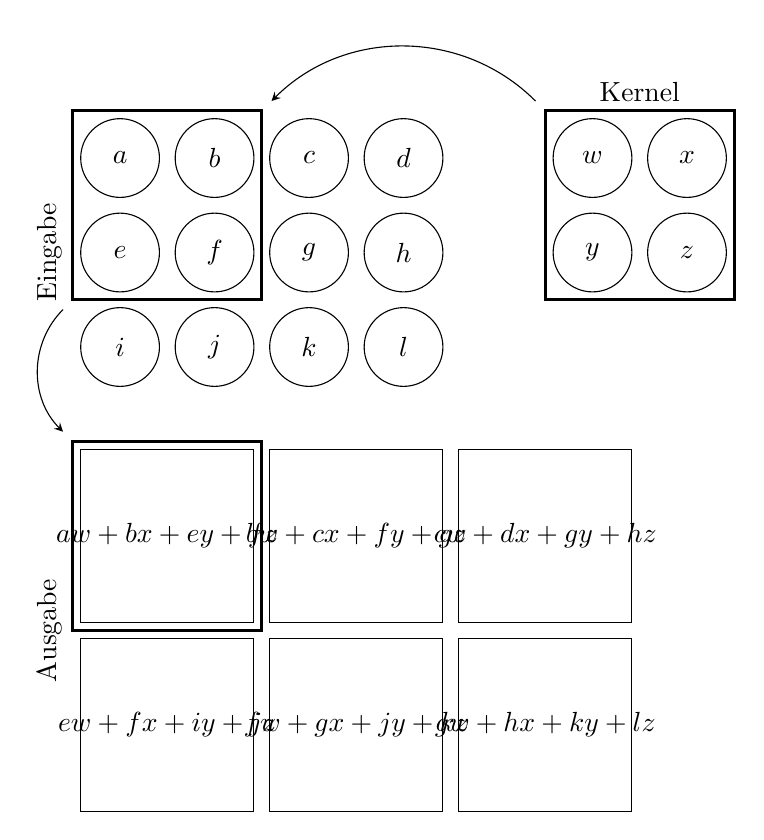
\begin{tikzpicture}[x=1.5cm, y=1.2cm, >=stealth]
			
			\foreach \m/\l [count=\y] in {1,2,3}
			\node [every neuron/.try, neuron \m/.try] (input-\m) at (0,2.5-\y) {};
			
			\foreach \m [count=\y] in {1,2,3}
			\node [every neuron/.try, neuron \m/.try ] (hidden1-\m) at (0.8,2.5-\y) {};
			
			\foreach \m [count=\y] in {1,2,3}
			\node [every neuron/.try, neuron \m/.try ] (hidden2-\m) at (1.6,2.5-\y) {};
			
			\foreach \m [count=\y] in {1,2,3}
			\node [every neuron/.try, neuron \m/.try ] (output-\m) at (2.4,2.5-\y) {};
			
			\foreach \m [count=\y] in {1,2}
			\node [every neuron/.try, neuron \m/.try ] (output-\m) at (4,2.5-\y) {};
			
			\foreach \m [count=\y] in {1,2}
			\node [every neuron/.try, neuron \m/.try ] (output-\m) at (4.8,2.5-\y) {};
			
			
			
			
			
			\foreach \m/\l [count=\y] in {0,1.6,3.2}
			\node[draw,rectangle,minimum width=2.2cm,minimum height=2.2cm] at (0.4+\m,-2.5) {};
			\foreach \m/\l [count=\y] in {0,1.6,3.2}
			\node[draw,rectangle,minimum width=2.2cm,minimum height=2.2cm] at (0.4+\m,-4.5) {};
			
			\node[] at (0.4,-2.5) {\Umbruch{$aw + bx + ey + fz$}};
			\node[] at (2,-2.5) {\Umbruch{$bw + cx + fy + gz$}};
			\node[] at (3.6,-2.5) {\Umbruch{$cw + dx + gy + hz$}};
			\node[] at (0.4,-4.5) {\Umbruch{$ew + fx + iy + jz$}};
			\node[] at (2,-4.5) {\Umbruch{$fw + gx + jy + kz$}};
			\node[] at (3.6,-4.5) {\Umbruch{$gw + hx + ky + lz$}};
			
			
			\node[] at (0,1.5) {$a$};
			\node[] at (0.8,1.5) {$b$};
			\node[] at (1.6,1.5) {$c$};
			\node[] at (2.4,1.5) {$d$};
			\node[] at (0,0.5) {$e$};
			\node[] at (0.8,0.5) {$f$};
			\node[] at (1.6,0.5) {$g$};
			\node[] at (2.4,0.5) {$h$};
			\node[] at (0,-0.5) {$i$};
			\node[] at (0.8,-0.5) {$j$};
			\node[] at (1.6,-0.5) {$k$};
			\node[] at (2.4,-0.5) {$l$};
			\node[] at (4,1.5) {$w$};
			\node[] at (4.8,1.5) {$x$};
			\node[] at (4,0.5) {$y$};
			\node[] at (4.8,0.5) {$z$};
			
			\node[rotate=90] at (-0.6,0.5) {Eingabe};
			\node[rotate=90] at (-0.6,-3.5) {Ausgabe};
			\node[] at (4.4,2.2) {Kernel};
			
			\node[] (S1) at (3.6,2){};
			\node[] (S2) at (1.2,2){};
			\node[] (S3) at (-0.4,-0.0){};
			\node[] (S4) at (-0.4,-1.5){};
			\node[very thick,draw,rectangle,minimum width=2.4cm,minimum height=2.4cm] at (0.4,-2.5) {};
			\node[very thick,draw,rectangle,minimum width=2.4cm,minimum height=2.4cm] at (4.4,1) {};
			\node[very thick,draw,rectangle,minimum width=2.4cm,minimum height=2.4cm] at (0.4,1) {};
			\draw [->, bend angle=45, bend right]  (S1) to (S2);
			\draw [->, bend angle=45, bend right]  (S3) to (S4);
		
			
			
			
			
		
			\end{tikzpicture}
			\caption{Prinzipielle Darstellung des Faltungsprozess. Adaptiert aus \cite{deeplearning}}
			\label{fig: faltung }
		\end{figure}
		
		Während der Konvolution, oder auch Faltung genannt, werden eingehende Daten in Filter, sogenannte Kernels, eingegeben. Abbildung \ref{fig: faltung } zeigt den prinzipiellen Vorgang der Faltung. Die Konfiguration des Kernels ist beispielhaft mit $w$, $x$, $y$ und $z$ dargestellt. Eingehend Datenpunkte sind hier mit den Buchstaben $a$ bis $l$ gekennzeichnet. Die Filter extrahieren bestimmte Merkmale je nach Konfiguration, wie im unteren Teil der Abbildung als Ausgabe dargestellt. So können verschiedene Schichten diverse Merkmale extrahieren. Die Ausgänge der Schichten üblicher, neuronaler Netzen sind mit jedem Eingang der folgenden Schicht verknüpft. Ein typischer Aufbau wurde bereits in Kapitel \ref{subsec: Eigenschaften von neuronalen Netzen} in Abbildung \ref{fig: neuronales netz } gezeigt. Wird bei derartigen Netzen eine Schicht mit $n$ Ausgaben und eine mit $m$ Eingaben verknüpft, werden $m \cdot n$ Parameter benötigt \cite{deeplearning}. Durch den Faltungsprozess wird diese Konnektivität eingeschränkt. Beispielsweise wird der Datenpunkt $b$ der Eingabe aus der Darstellung \ref{fig: faltung } lediglich in zwei von sechs Datenpunkten der Ausgabe berücksichtigt. Die Ausmaße der eingeschränkten Konnektivität lassen sich in der folgenden Abbildung \ref{fig: eingeschränkte konnektivität} verdeutlichen. Die Eingabepunkte $x_n$ geben je nach Netzart ihre Informationen an alle oder benachbarten Ausgabepunkte $s_n$ weiter. Die Einschränkung der Konnektivität hängt von der Dimension des Kernels ab. Folglich nehmen CNNs deutlich weniger Speicher ein im Vergleich zu herkömmlichen KNNs \cite{deeplearning}. Gleichzeitig wird durch die Faltung eine höhere Statistische Effizient erreicht \cite{deeplearning}.\\
		
	
			\tikzset{%
			every neuron/.style={
				circle,
				draw,
				minimum size=1cm
			},
			neuron missing/.style={
				draw=none, 
				%scale=4,
				%rotate=90,
				%yshift=1,
				%text height=0.333cm,
				%execute at begin node=\color{black}$\cdots$
			},
		}
		\begin{figure}[H]
			\centering
			
			
			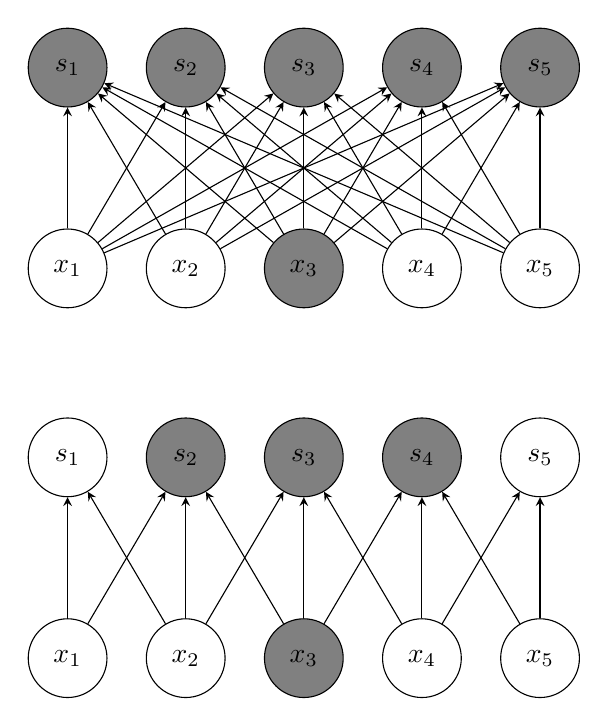
\begin{tikzpicture}[x=1.5cm, y=1.5cm, >=stealth]
			
			\foreach \m/\l [count=\y] in {1,2,3,4,5}
			\draw[gray,fill=gray](0+\y,2.5)circle(14pt);
			
			\foreach \m/\l [count=\y] in {2,3,4}
			\draw[gray,fill=gray](0+\m,-0.8)circle(14pt);
			
			\draw[gray,fill=gray](3,0.8)circle(14pt);
			\draw[gray,fill=gray](3,-2.5)circle(14pt);
			
			\foreach \m/\l [count=\y] in {1,2,3,4,5}
			\node [every neuron/.try, neuron \m/.try] (eins-\m) at (0+\y,2.5) {$s_\y$};
			
			\foreach \m/\l [count=\y] in {1,2,3,4,5}
			\node [every neuron/.try, neuron \m/.try] (zwei-\m) at (0+\y,0.8) {$x_\y$};
			
			\foreach \m/\l [count=\y] in {1,2,3,4,5}
			\node [every neuron/.try, neuron \m/.try] (drei-\m) at (0+\y,-0.8) {$s_\y$};
			
			\foreach \m/\l [count=\y] in {1,2,3,4,5}
			\node [every neuron/.try, neuron \m/.try] (vier-\m) at (0+\y,-2.5) {$x_\y$};
			
		
			\foreach \m [count=\x] in {1,2,3,4,5}
			\foreach \l [count=\i] in {1,2,3,4,5}
			\draw [<-] (eins-\i) -- (zwei-\x)
			node [] {};
			
			
			\draw [<-] (drei-1) -- (vier-1);
			\draw [<-] (drei-1) -- (vier-2);
			\draw [<-] (drei-2) -- (vier-1);
			\draw [<-] (drei-2) -- (vier-2);
			\draw [<-] (drei-2) -- (vier-3);
			\draw [<-] (drei-3) -- (vier-2);
			\draw [<-] (drei-3) -- (vier-3);
			\draw [<-] (drei-3) -- (vier-4);
			\draw [<-] (drei-4) -- (vier-3);
			\draw [<-] (drei-4) -- (vier-4);
			\draw [<-] (drei-4) -- (vier-5);
			\draw [<-] (drei-5) -- (vier-4);
			\draw [<-] (drei-5) -- (vier-5);
			
		
			\end{tikzpicture}
			\caption{deep learning}
			\label{fig: eingeschränkte konnektivität}
		\end{figure}
		
		Als Parameterverteilung bezeichnet man die Nutzung eines Parameters pro Funktion eines Netzes \cite{deeplearning}. Bei grundlegenden künstlichen neuronalen Netzen wird jede Eingabe eines Neurons, wie in Kapitel \ref{subsec: Eigenschaften von neuronalen Netzen}, mit einem Gewicht verrechnet  \cite{deeplearning}. Wie bereits beschrieben, wird bei CNNs ein Kernel pro Schicht für die Merkmalsextraktion verwendet. Dies führt zu deutlich weniger Speicheraufwand, da das Netz lediglich die Kernels abspeichert statt aller Gewichte pro Neuron.\\
		
		Die äquivariante Darstellung bezieht sich auf die Auswirkung der Ausgabe bei einer Änderung der Eingabedaten. Die Konvolution erzeugt eine zweidimensionale Karte, die sogenannte \textit{Featuremap} in der Merkmale eines Bildes eingetragen sind. Wird ein Objekt in dem eingegebenen Bild des CNNs bewegt, verändert sich die Merkmalskarte im selben Maße. ...\\
		
		
		Beim \textit{Pooling} werden die stärksten Merkmale der eingehende Daten weitergegeben \cite{deeplearning}. Kleine Änderungen der Eingabewerte haben durch \textit{Pooling} keinen oder einen kleinen Einfluss auf die Ausgabe. Ein Beispiel hierfür liefert die folgende Darstellung \ref{fig: Pooling}.\\
		
				\tikzset{%
			every neuron/.style={
				circle,
				draw,
				minimum size=1cm
			},
			neuron missing/.style={
				draw=none, 
				%scale=4,
				%rotate=90,
				%yshift=1,
				%text height=0.333cm,
				%execute at begin node=\color{black}$\cdots$
			},
		}
		\begin{figure}[H]
			\centering
			
			
			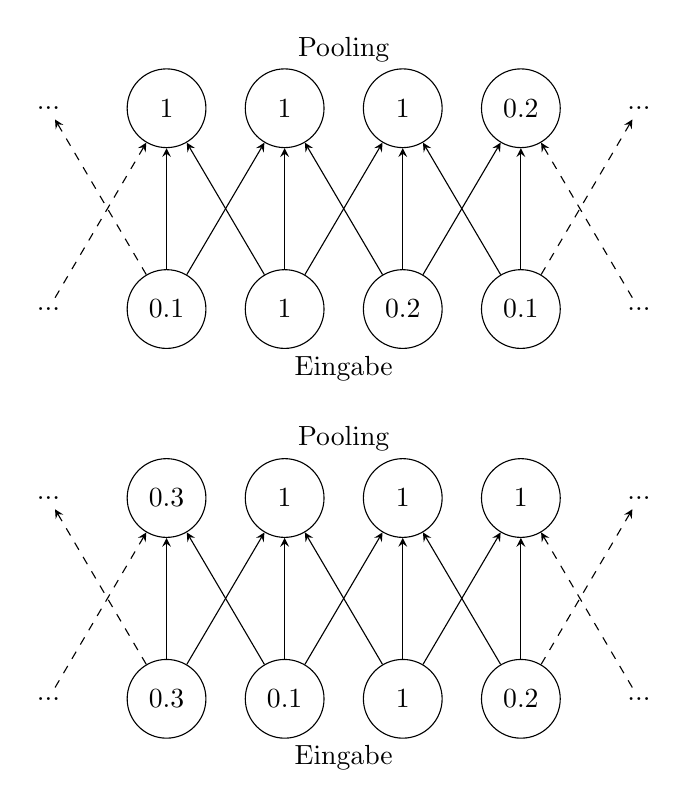
\begin{tikzpicture}[x=1.5cm, y=1.5cm, >=stealth]
			
			%\foreach \m/\l [count=\y] in {1,2,3,4}
			%\draw[gray,fill=gray](0+\y,2.5)circle(14pt);
			
			%\foreach \m/\l [count=\y] in {2,3,4}
			%\draw[gray,fill=gray](0+\m,-0.8)circle(14pt);
			
			%\draw[gray,fill=gray](3,0.8)circle(14pt);
			%\draw[gray,fill=gray](3,-2.5)circle(14pt);
			
			\foreach \m/\l [count=\y] in {1,2,3,4}
			\node [every neuron/.try, neuron \m/.try] (eins-\m) at (0+\y,2.5) {};
			
			\foreach \m/\l [count=\y] in {1,2,3,4}
			\node [every neuron/.try, neuron \m/.try] (zwei-\m) at (0+\y,0.8) {};
			
			\foreach \m/\l [count=\y] in {1,2,3,4}
			\node [every neuron/.try, neuron \m/.try] (drei-\m) at (0+\y,-0.8) {};
			
			\foreach \m/\l [count=\y] in {1,2,3,4}
			\node [every neuron/.try, neuron \m/.try] (vier-\m) at (0+\y,-2.5) {};
			
			
%			\foreach \m [count=\x] in {1,2,3,4}
%			\foreach \l [count=\i] in {1,2,3,4}
%			\draw [<-] (eins-\i) -- (zwei-\x)
%			node [] {};
			
			\node[] (1) at (1,2.5){$1$};
			\node[] (1) at (2,2.5){$1$};
			\node[] (1) at (3,2.5){$1$};
			\node[] (1) at (4,2.5){$0.2$};
			
			\node[] (1) at (1,0.8){$0.1$};
			\node[] (1) at (2,0.8){$1$};
			\node[] (1) at (3,0.8){$0.2$};
			\node[] (1) at (4,0.8){$0.1$};
			
			\node[] (1) at (1,-0.8){$0.3$};
			\node[] (1) at (2,-0.8){$1$};
			\node[] (1) at (3,-0.8){$1$};
			\node[] (1) at (4,-0.8){$1$};
			
			\node[] (1) at (1,-2.5){$0.3$};
			\node[] (1) at (2,-2.5){$0.1$};
			\node[] (1) at (3,-2.5){$1$};
			\node[] (1) at (4,-2.5){$0.2$};
			
			\node[] (1) at (2.5,3){Pooling};
			\node[] (1) at (2.5,0.3){Eingabe};
			\node[] (1) at (2.5,-0.3){Pooling};
			\node[] (1) at (2.5,-3){Eingabe};
			
			\node[] (S1) at (5,2.5){...};
			\node[] (S2) at (0,2.5){...};
			\node[] (S3) at (5,0.8){...};
			\node[] (S4) at (0,0.8){...};
			\node[] (S5) at (5,-0.8){...};
			\node[] (S6) at (0,-0.8){...};
			\node[] (S7) at (5,-2.5){...};
			\node[] (S8) at (0,-2.5){...};
			\draw [<-] (eins-1) -- (zwei-1);
			\draw [<-] (eins-1) -- (zwei-2);
			\draw [<-] (eins-2) -- (zwei-1);
			\draw [<-] (eins-2) -- (zwei-2);
			\draw [<-] (eins-2) -- (zwei-3);
			\draw [<-] (eins-3) -- (zwei-2);
			\draw [<-] (eins-3) -- (zwei-3);
			\draw [<-] (eins-3) -- (zwei-4);
			\draw [<-] (eins-4) -- (zwei-3);
			\draw [<-] (eins-4) -- (zwei-4);
			\draw [<-,dashed] (S1) -- (zwei-4);
			\draw [<-,dashed] (S2) -- (zwei-1);
			\draw [<-,dashed] (eins-1) -- (S4);
			\draw [<-,dashed] (eins-4) -- (S3);
			
			\draw [<-] (drei-1) -- (vier-1);
			\draw [<-] (drei-1) -- (vier-2);
			\draw [<-] (drei-2) -- (vier-1);
			\draw [<-] (drei-2) -- (vier-2);
			\draw [<-] (drei-2) -- (vier-3);
			\draw [<-] (drei-3) -- (vier-2);
			\draw [<-] (drei-3) -- (vier-3);
			\draw [<-] (drei-3) -- (vier-4);
			\draw [<-] (drei-4) -- (vier-3);
			\draw [<-] (drei-4) -- (vier-4);
			\draw [<-,dashed] (S5) -- (vier-4);
			\draw [<-,dashed] (S6) -- (vier-1);
			\draw [<-,dashed] (drei-1) -- (S8);
			\draw [<-,dashed] (drei-4) -- (S7);
			
			
			
			\end{tikzpicture}
			\caption{deep learning}
			\label{fig: Pooling}
		\end{figure}
		
		In Abbildung \ref{fig: Pooling}a werden beispielhaft die stärksten Merkmale der Eingangsdaten durch das \textit{Pooling} weitergeleitet. Obwohl in der unteren Darstellung alle Eingangsdaten um eine Stelle nach rechts verschoben wurden, hält das Verfahren zwei Merkmale konstant. Dies untermauert die Motivation der äquivrianten Darstellung.
		
		/bild Klassifikation\\
		
		Für die Klassifikation der Daten setzen sich die letzten Schichten meist aus einer oder mehrerer vollständig verbundenen Schichten und einer \textit{Softmax}-Schicht zusammen \cite{deeplearning}. Die vollständig verbundene Schicht gibt einen Vektor mit $K$ Elementen aus, wobei $K$ für die Anzahl der ausgegebenen Klassen steht. Eine \textit{Softmax}-Funktion repräsentiert grundlegend eine Wahrscheinlichkeitsverteilung des Eingabevektors $K$. Durch die \textit{Softmax}-Schicht wird der Vektor in einem Zahlenbereich von Null bis Eins transformiert. Die Summe aller Elemente des Vektors ergeben 1. Jedes Element wird als Konfidenz der jeweiligen Klasse interpretiert. An dieser Stelle sind alle Daten vollständig bearbeitet und werden als Vektor aus dem CNN ausgegeben. In Abbildung \ref{fig: cnn easy} wird die Funktionsweise eines Faltungsnetzwerks anhand eines Minimalbeispiels dargestellt.\\
		
		\begin{figure}[H]
			\centering
			\begin{tikzpicture}[node distance=4em]
			\node[3d matrix] (mat1){ 
				0 & 0 & 1 & 1 & 0 & 0 & -1 & -1 & 0 & 0 \\
			};
			\node[3d matrix,above=of mat1] (mat2){ 
				0 & 0 & 1 & 1 & 0 & 0 & -1 & -1 & 0 & 0\\
				0 & 0 & -1 & -1 & 0 & 0 & 1 & 1 & 0 & 0\\
			};
			\node[3d matrix,above=of mat2] (mat3){ 
				0 & 1 & 0 & -1 & 0 \\
				0 & -1 & 0 & 1 & 0 \\
			};
			\node[3d matrix,above=of mat3] (mat4){ 0 & -4 & 0 \\};
			\node[3d matrix,above=of mat4] (mat5){ 4 & -4 \\};
			\node[3d matrix,above=of mat5] (mat6){ 0.99 & 0.01 \\};
			\node[] (S1) at (-4,0) {Eingabe};
			\node[] (S2) at (-4,1.1) {Faltung};
			\draw[dashed](S2)--(0.5,1.1);
			\node[] (S3) at (-4,3.9) {Pooling};
			\draw[dashed](S3)--(0.5,3.9);
			\node[] (S4) at (-4,6.6) {Faltung};
			\draw[dashed](S4)--(0.5,6.6);
			\node[] (S5) at (-4,8.8) {Vollständig verbundene Schicht};
			\draw[dashed](S5)--(0.5,8.8);
			\node[] (S6) at (-4,11.1) {Softmax};
			\draw[dashed](S6)--(0.5,11.1);
			\draw[-{Latex[bend]}] (mat1.east) to[out=0,in=0] 
			coordinate[near end](aux1) ([xshift=1ex]mat2-1-10.east);
			\path (aux1) node[right,above right,3d matrix]{-1 & 0 & 1\\}; 
			\draw[-{Latex[bend]}] (mat1.east) to[out=0,in=0] ([xshift=1ex]mat2-2-10.east);
			\draw[very thick,-Latex] (mat1) -- coordinate[midway,right=2em] (aux2) (mat2);
			\path (aux2) node[right,3d matrix] (mat1a){1 & 0 & -1 \\};
			\draw[very thick,-Latex] (mat2) -- (mat3);
			\draw[very thick,-Latex] (mat3) -- (mat4)
			coordinate[midway,right=1em] (aux3);
			\path (aux3) node[right,3d matrix] (mat3a){-1 & 0 & 1 \\
				1 & 0 & -1\\};
			\foreach \X in {1,2,3} {\foreach \Y in {1,2}
				{\draw[-latex] (mat4-1-\X) -- (mat5-1-\Y);}}
			\draw[very thick,-Latex] (mat5) -- (mat6);
			\end{tikzpicture}
			\caption{https://tex.stackexchange.com/questions/519268/write-convolutional-neural-networks-using-tikzg}
			\label{fig: cnn easy}		
		\end{figure}
		
		Die Artenvielfalt der CNNs ist sehr breit gefächert. Jedes Netzwerk unterscheidet sich in der jeweiligen Architektur der Schichten. Durch die Änderung verschiedener Parameter, beispielsweise bei der Faltung oder beim Pooling, können CNNs im Einsatz jeweils anders reagieren. Hierbei entscheidet man bei der Auswahl des Modells häufig unter den Gesichtspunkten Bearbeitungszeit, Genauigkeit und je nach Anwendungsfall spielt der Speicherplatz ebenfalls eine große Rolle.\\
		
			
		
		Auf dem ALF werden je Kamera 10 Bilder in der Sekunde eingelesen. Folglich wird eine Netzarchitektur verwendet, die in der Lage ist mindestens 20 Bilder zu verarbeiten. Für eine zukünftige Auslagerung auf ein eingebettetes System soll das neuronale Netz nach den dafür notwendigen Aspekten entwickelt werden. Hinsichtlich der genannten Aspekte wird im Zuge dieser Arbeit ein KNN mit der MobileNet Architektur und dem \textit{Single Shot Detector} (SSD) Framwork verwendet. Die Grundlage der Auswahl wird mithilfe der Paper \textit{MobileNets: Efficient Convolutional Neural Networks for  Mobile Vision Applications} \cite{mobilenets} und \textit{The Implementation of CNN-based Object Detector on ARM Embedded Platforms} \cite{embedded} begründet.\\
		
		Die \textit{MobileNet} Architektur ermöglicht im Vergleich zu anderen Lösung zur Merkmalsextraktion den gesuchten Spagat zwischen Schnelligkeit, Genauigkeit und Größe des Netzes \cite{mobilenets}. Das Hauptmerkmal ist der Aufbau der Konvolutionsschichten, der zu den genannten Eigenschaften in der Praxis führt \cite{mobilenets} \cite{embedded}. Vergleichsmessungen zu anderen Architekturen werden in den erwähnten Paper durchgeführt. Der \textit{Single Shot Detector} dient als Klassifikator und zeichnet sich besonders durch seine Schnelligkeit aus \cite{ssd}. Er erreicht eine höhere Genauigkeit als andere state-of-the-art Lösungen wie zum Beispiel \textit{Faster R-CNN} \cite{fastercnn} und ist zudem dreimal schneller\cite{ssd}.
		
	
	
		
	

			
	\section{Zustandsautomat}
	\label{sec: Zustandautomat}
	Die Idee der Nutzung eines Zustandsautomaten oder auch endlicher Automat (EA) ergab sich im Laufe der Entwicklungsphase. In der in Kapitel ... erwähnten Bachelorarbeit werden diverse Modi beschrieben, die den Aufruf von unterschiedlichen ROS-Knoten vorraussetzen. Aufgrund der Analogie zwischen den beschriebenen Modi und der Zustände eines Zustandsautomaten wird die Nutzung eines solchen Automaten begründet. Im Folgenden wird auf die Eigenschaften eines endlichen Automats eingegangen.\\
	
	Im Allgemeinen geht es bei einem Zustandsautomaten um die Beschreibung der Zustände (engl. States) eines Objekts. Dabei stellt das Objekt meist das Gesamtsystem dar, etwa ein Getränkeautomat oder wie dieser Arbeit autonomes Fahrzeug. States sind durch Bedingungen verknüpft und lösen während sogenannter Ereignisse eine Transition aus, die den Wechsel des Zustands ausübt. Weiterhin Bilden die Zustände in ihrer Gesamtheit den Lebenszyklus des Objekts. Ein Getränkeautomat befindet sich bekanntermaßen beim Eintreffen eines Kunden in einer Art Bereitschaft. Übertragen auf die Theorie eines Zustandsautomaten wäre dies ein Bereitschaftszustand. Die Auswahl des Getränks und die Eingabe des entsprechenden Geldbetrags können beispielhaft als Ereignisse interpretiert werden. Somit wird ein Transition durchgeführt und der Zustand der Getränkeausgabe wird losgetreten. Wurde das Getränk ausgegeben und entnommen, geschieht der Wechsel in den Bereitschaftszustand und der beschriebene Zyklus ist komplettiert.\\
	
	Seit dem Bestehen der endlichen Automaten haben sich in der Praxis zwei Typen durchgesetzt. Mealy und Moore Automaten unterscheiden sich grundlegend in ihrem Verhalten und können durch folgende Gleichungen beschrieben werden.\\
	
	\begin{equation}
		\alpha_{t+1}=\phi(\zeta_t,\alpha_t)\text{    mit    t}\in\mathbb{N}
		\label{eq: transferfct}
	\end{equation}

	\begin{equation}
		\gamma_t=\psi(\zeta_t,\alpha_t)\text{    mit    t}\in\mathbb{N}
		\label{eq: transferfct}
	\end{equation}
	\\
	In den Gleichung ... beschreibt $\varphi$ die Transitionsfunktion und $\psi$ die Ausgabefunktion des Mooreautomats. Die Transition steht in Abhängigkeit von $\zeta_t $, die aktuelle Eingabe, und $\alpha_t$, der aktuelle Zustand selbst. Mithilfe der Transitionsfunktion lässt sich der Zustand bestimmen, der im folgenden Zeitschritt $t$ angestrebt werden soll. Der Ausgang des Moore Automaten wird durch die Ausgangsfunktion $psiup$ berechnet. Diese hängt genau wie die Transitionsfunktion von der Eingabe und dem Zustand zum Zeitpunkt $t$ ab. \\
	
	\begin{equation}
		\alpha_{t+1}=\phi(\zeta_t,\alpha_t)\text{    mit    t}\in\mathbb{N}
		\label{eq: transferfct}
	\end{equation}
	
	\begin{equation}
		\gamma_t=\psi(\alpha_t)\text{    mit    t}\in\mathbb{N}
		\label{eq: transferfct}
	\end{equation}
	\\
	
	Beim Vergleich der beiden Gleichungen ... und ... stellt sich heraus, dass die Ausgangsfunktion $psi$ in der Beschreibung des Verhaltens eines endlichen Automaten durch Moore lediglich vom Ausgang zum Zeitpunkt $t$ abhängig ist.
	
	Eine Unterkategorie der Finiten Automaten ist der Hierarchische Zustandsautomat. Die Besonderheit hierbei ist die Zusammensetzung aller vorangegangenen Zustände eines aktiven Zustands. Diese sind bei der hier beschriebenen hierarchisch aufgebauten Maschine nämlich ebenfalls aktiv. So besteht die Möglichkeit eines aufeinander aufbauenden Endzustands. 
	
	
		
		
	\section{Bestimmung von Positionskoordinaten}
		Während der Durchführung autonomer Fahr- bzw. Logistikaufgaben können diverse Probleme auftreten, die eine erfolgreiche Bearbeitung verhindern können. Beispielsweise können Türen geschlossen sein oder Gegenstände die geplante Route blockieren. Da das ALF nicht über die technischen Möglichkeiten besitzt derartige Problemstellungen zu lösen, müssen Menschen Abhilfe schaffen. Für diese Zwecke ist die Kenntnis über die letzte Position der erfassten Personen realtiv zur statischen Karte  notwendig. Anstehende Fahraufgaben werden, bedingt durch das Vorgängerprojekt, mithilfe des Robot Operating Systems gelöst. Personen können folglich als Position in das ROS Netzwerk veröffentlicht. Dies ermöglicht dem Roboter die veröffentlichten Positionen anzufahren. Die Eintragung der Position in die statische Karte setzt die Beschreibung der Position als Koordinaten vorraus. Für die Bestimmung der Positionskoordinaten wird ein zweidimensionales Bild und die dazugehörigen Tiefeninformationen genutzt. Die Koordinate xloc beschreibt hier die longitudinale Entfernung von der Kamera zur Person. Eingehende laterale Distanzen werden durch die Koordinate yloc dargestellt.
		
	\begin{figure}[H]
		\centering
			\begin{tikzpicture}[]
				\draw[<->] (-5,0) -- (5,0) node[right] {$y$};
				\draw[->] (0,-1.2) -- (0,7) node[above] {$x$};

				\draw[thin,-] (0,0) -- (4,6) node[above] {$f_{r}$};
				\draw[thin,-] (0,0) -- (-4,6) node[above] {$f_{l}$} ;
				\draw[densely dotted] (1,1.5) -- (-1,1.5) node[left] {$Bild$};
				\filldraw [black] (1.5,4.5) circle (2pt);
				\draw[dashed] (0,0) -- (1.5,4.5) node[above] {$Objekt$};
				\draw[very thick] (0,4.5) -- (1.5,4.5) node[left] {};
				\draw[very thick] (0,0) -- (0,4.5) node[left] {};
				\draw[very thick]  (0,3) node[left] {$x_{loc}$};
				\draw[very thick]  (0.75,4.0) node[above] {$y_{loc}$};
				\draw[very thick]  (0,1) node[left] {$x_{f}$};
			\end{tikzpicture}
		
		\caption{(a) Die Abbildung zeigt die Übergangsfunktion $h(t)$ eines Verzögerungsglieds erster Ordnung als Antwort auf die sprungförmige Eingangsgröße $u(t)$ mit $\hat{u}=1$. (b) Die Impulsantwort auf das Eingangssignal $\delta(t)$. Zwischen den Funktionen $h(t)$ und $g(t)$ besteht der Zusammenhang \mbox{$g(t)=\frac{\mathrm d}{\mathrm d t}\:h(t)$}.}
		\label{fig: antworten}
	\end{figure}

	\section{Schnittstelle zwischen ROS und Python}
	     
	

